\chapter{Testing}
\section{Overall Approach to Testing}
stuff here please

\section{Client Testing}
\subsection{User Interface Testing}
The Android SDK comes bundled with a number of automated user interface testing tools\footnote{http://developer.android.com/tools/testing/testing\_ui.html}. These functional tests allow for automated testing of component behaviour as well as responding correctly to user actions. This projects interface contained very few components that actually performed very little functionality. One possible candidate for such testing could have been the map views response to using the zoom controls. This however was considered to trivial, along with any other possible test cases, that the time was not invested to automate this process. These functionalities however formed a key role in using the application so would have been quickly picked up by both developer interaction and manual testing.

\subsection{Manual Testing}


\section{Server Testing}
\subsection{Automated Testing}
While developing portions of the server program it would have been impractical to use the production client as a primary testing tool. For this reason a small testing suite was created in Python which can be seen in Appendix \ref{server_testing}. This tool create an easy to use command line interface program that could impersonate a natively running Android client.

\begin{figure}[H]
  \centering
   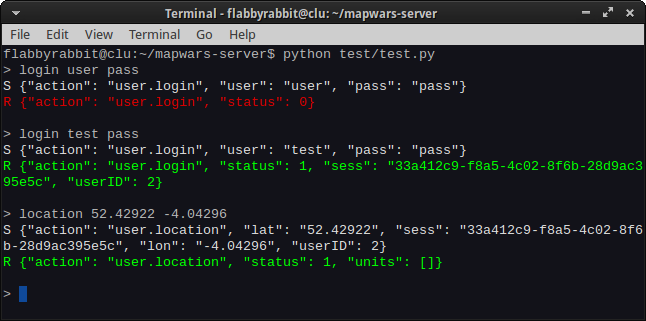
\includegraphics[width=0.5\textwidth]{Images/test.png}
  \caption{Isometric view of main game screen,\\showing separation between components}
  \label{fig:isogui}
\end{figure}

\subsection{Stress Testing}
5k per unit, linear ... doesn't go down again, clearly
1%



\section{User Testing}

\renewcommand{\arraystretch}{1.5}
\begin{tabular}{l  p{11cm}}
	\hline
	Name: & Peter Maynard \\
	\hdashline
	Device: & Sony Ericsson ST25i \\
	\hdashline
	Android version: & 2.3.7 Gingerbread \\
	\hdashline
	Screen size: & 3.5 inches, 480 x 854 pixels \\
	\hdashline
	Comments: & Had fun playing around with generating units and fighting them. There was a limited amount of units which was a shame, but can see the potential and look forward to playing with more users. \\
	\hline
\end{tabular}

\begin{tabular}{l  p{11cm}}
	\hline
	Name: & Anika Rusnakova \\
	\hdashline
	Device: & Motorola Xoom 2 ME \\
	\hdashline
	Android version: & 4.0.4 Ice Cream Sandwich \\
	\hdashline
	Screen size: & 8.2 inches, 1280 x 800 pixels \\
	\hdashline
	Comments: & Good yeah I guess good yeah I guess good yeah I guess good yeah I guess good yeah I guess \\
	\hline
\end{tabular}